\chapter{Monitoring DLAKaApp}
\label{cha:first_solution}

This chapter applies the extended UME approach from Chapter \ref{cha:concept}
to the BestRentalPoC by extending its story. This answers the second research question.
The name of the developed monitoring software is SPMonitor. The
chapter is oriented along the different phases of software development. First,
Section \ref{sec:story} extends the story of BestRentalPoC. Then follow
the analysis of SPMonitor in Section \ref{sec:analysis}, the design in Section
\ref{sec:design}, and the implementation and deployment in Section
\ref{sec:impl_and_deployment}.

\section{Story}
\label{sec:story}

The development of SPMonitor will be based on the following story.
This extends the story of the BestRentalPoC.

The DrivingLicenseAuthorityKarlsruhe (DLAKa) wants to provide citizens with
digital driving licenses, which can, for example, be used by citizens to prove
to a car rental company that they possess a valid driving license. They hire
the company ServiceProvider (SP) to develop and operate the system necessary
for issuing and verifying digital driving licenses. The contract specifies an
initial payment for the development of the system and afterward a yearly fee
for the operation of the system. After receiving the contract from DLAKa, SP
starts to design the system for DLAKa. Because SP has to operate the system on
a fixed yearly budget, they want to monitor the performance of the system to
identify parts with excessive resource usage, which incur additional costs.
They identify the memory usage of the system as a technical metric that should
be monitored. This metric will be called MemUse (Memory Usage). Additionally,
DLAKa has asked SP to provide the capability of monitoring business
metrics for them. DLAKa wants to know how many digital driving licenses
are being issued. This metric will be called numDDL (Number of Issued Digital
Driving Licenses). To monitor both technical and business metrics, SP designs
the ServiceProviderMonitor (SPMonitor) as a part of the system for DLAKa
which will provide all functionality for monitoring the specified metrics.

\section{Analysis}
\label{sec:analysis}

The following section will provide an analysis of SPMonitor based on the
story above. Firstly, use cases are derived from the story above.
These use cases are then used to derive capabilities and requirements for
SPMonitor. This will be followed by defining the metrics that SPMonitor will
collect. Finally, SPMonitor will be analyzed regarding its integration with
DLAKaApp and modifications that might have to be made in DLAKaApp.

\subsection{Use Cases}

Based on the story, three use cases for SPMonitor were derived: Inspect
Metric, Configure Metric, and Assign Permissions. The use case Inspect Metric
is concerned with the presentation of monitoring data to the users of
SPMonitor. The use case Configure Metric describes how metrics will be added to
SPMonitor. Lastly, the use case Assign Permissions covers the control of access
to the collected data. The relation of these use cases can be seen in Figure
\ref{fig:use_case_diagram_spmonitor} as a use case diagram.

\begin{figure}[tb]
  \centering
  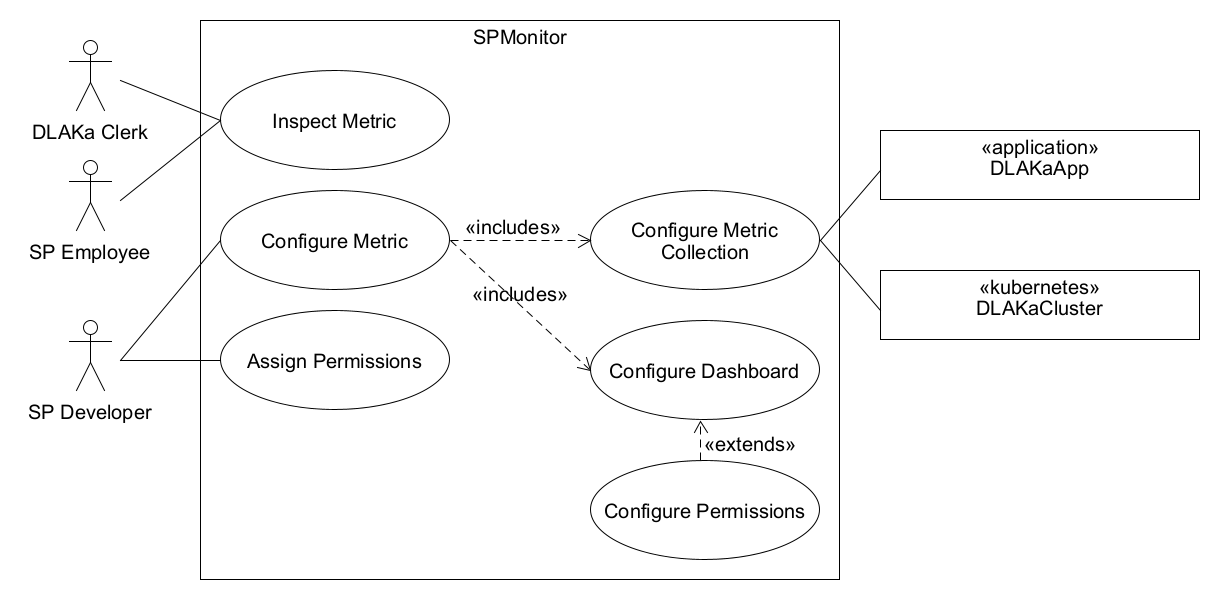
\includegraphics[width=\textwidth]{figures/6.1_use_case_spmonitor.png}
  \caption{Use Case Diagram: SPMonitor}
  \label{fig:use_case_diagram_spmonitor}
\end{figure}

The use case description of Inspect Metric can be seen in Listing
\ref{lis:use_case_description_inspect_metric}. This use case has two primary
actors DLAKa Clerk and SP Employee as seen in line 1. Both of these primary actors are users of
SPMonitor who differ in their assigned roles. A user of SPMonitor can have one
of two roles. Firstly, a user could work for DLAKa and thus have the role DLAKa
Clerk. The other possibility is that the user could work for SP and have the
role SP Employee. Due to possible privacy concerns, each user can only have one
of these two roles. Based on their role they will be able to access different
dashboards which contain different data. The preconditions of this use case are
that a metric has been configured for collection and that a dashboard has been
set up that the user wants to access as seen in lines 5 to 7. A dashboard presents related monitoring
data as a collection of graphs. The flow of the use case is described in lines 9 to 12
After the user selects a dashboard, SPMonitor will retrieve the stored values for the dashboard and display them in graphs.
The alternative flow of the use case can be seen in lines 14 to 16.
Alternatively, if the user does not have permission to access the
dashboard, SPMonitor will not open the dashboard for the user.
The information requirement for the use case as described in lines 18 and 19 is that
the metric that the user wants to access has data that is available in SPMonitor.

\begin{lstlisting}[caption = {Use Case Description: Inspect Metric}, label = {lis:use_case_description_inspect_metric}, style = kit-cm, language=]
Title: Inspect Metric

Primary Actors: DLAKa Clerk, SP Employee

Preconditions:
- SPMonitor has a metric configured
- SPMonitor has a dashboard for the metric configured

Flow:
1. The user opens a dashboard for a metric
2. SPMonitor retrieves all stored values for that metric
3. SPMonitor displays the values to the user in the dashboard

Alternative Flows:
1a. The user does not have the permission to access the dashboard
2a1. The user can not open the dashboard

Information Requirements:
- Values for the metric
\end{lstlisting}

The use case description of the Configure Metric use case can be seen in
Listing \ref{lis:use_case_description_configure_metric}. This use case has one
primary actor who works for SP as a developer, called SP Developer as seen in line 3.
Additionally, the use case has two secondary actors the DLAKaApp and the
DLAKaCluster as seen in line 4. DLAKaApp is the application that is being monitored and
DLAKaCluster is a Kubernetes cluster that represents DLAKaApp's runtime
environment. The flow of the use case is described in lines 6 to 9.
First SP Developer configures the collection of a metric. This
involves setting up either the DLAKaApp or DLAKaCluster to emit the metric that
should be collected and then setting up SPMonitor to collect that metric. After
SPMonitor collects the metric, SP Developer configures a dashboard for that
metric. After the graphs for the dashboard have been created SP Developer
selects which of the two roles DLAKa Clerk or SP Employee can access the
dashboard.

\begin{lstlisting}[caption = {Use Case Description: Configure Metric}, label = {lis:use_case_description_configure_metric}, style = kit-cm, language=]
Title: Configure Metric

Primary Actor: SP Developer
Secondary Actors: DLAKaApp, DLAKaCluster

Flow:
1. SP Developer configures the collection of a metric
2. SP Developer configures a dashboard for the metric
3. SP Developer configures the permissions of the dashboard
\end{lstlisting}

The use case description of the Assign Permissions use case can be seen in
Listing \ref{lis:use_case_description_assign_permissions}. This use case has SP
Developer as its primary actor as seen in line 3. The only precondition of this use case is that SPMonitor must have a
registered user which is described in lines 5 and 6. 
The flow of the use case is described in lines 8 and 9.
SP Developer assigns this registered user either the role
DLAKa Clerk or SP Employee depending on which organization the user belongs to.

\begin{lstlisting}[caption = {Use Case Description: Assign Permissions}, label = {lis:use_case_description_assign_permissions}, style = kit-cm, language=]
Title: Assign Permissions

Primary Actor: SP Developer

Preconditions:
- SPMonitor has a registered user

Flow:
1. SP Developer assigns a user permission to access a dashboard
\end{lstlisting}

\subsection{Metrics Definition}

In this section, the two metrics MemUse and numDDL will be defined.
The definitions of these two metrics will use the Metric Definition artifact
from the extended UME approach developed in Chapter \ref{cha:concept}.
The definition of the MemUse metric in the form of a
Metric Definition can be seen in Listing \ref{lis:metric_definition_memUse}.
As the story in Section \ref{sec:story} stated, the purpose of the MemUse metric
is to identify services within the DLAKaApp that use excessive amounts of resources
which incur high operating costs.
The MemUse metric combines the amount of main memory currently being used by each service
into an additional value that is the sum of all the service's memory usage. This sum
is an aggregation which makes the MemUse an aggregated metric.
Because the amount of memory being used captures the current state of the DLAKaApp,
the MemUse metric is also a technical metric. Together, this makes the MemUse metric
an aggregated technical metric. The visual representation of the MemUse metric
consists of two different types of visualization: a line graph in which the historical
development of the metric can be seen and a gauge that displays the metric's current value
within the ranges defined in Listing \ref{lis:metric_definition_memUse}.
Both of these visualizations are used for each service's memory usage
and the total memory usage of DLAKaApp.

\begin{figure}[tb]
\begin{lstlisting}[caption = {Metric Definition: MemUse}, label = {lis:metric_definition_memUse}, style = kit-cm, language=]
Name: MemUse

Purpose:
Capture the amount of main memory being used by DLAKaApp and SPMonitor
to find services with excessive resource usage to prevent high operating costs.

Type: Aggregate, Technical

Values:
  - For each service in the DLAKaApp: the amount of main memory
    that is currently being used in bytes
  - Total: Sum over the values of all services

Visual Representation:
  Per Value:
  - 1: Line Graph with time as the x-axis and the current metric value as the y-axis.
  - 2: Gauge with different colors for the different ranges of the metric.

Ranges:
  Per Value:
  - Ok: Value < 3 GB
  - Warning: 3 GB < Value < 4 GB
  - Critical: Value > 4 GB
\end{lstlisting}
\end{figure}

The definition of the numDDL metric in the form of a
Metric Definition can be seen in Listing \ref{lis:metric_definition_numDDL}.
As the story in Section \ref{sec:story} stated, the purpose of the numDDL is to capture how many
digital driving licenses were issued by the DLAKaApp so that DLAKa can evaluate
the success of the DLAKaApp. Because the numDDL metric only uses a single value,
the number of issued digital driving licenses, it is an elementary metric.
Additionally, the numDDL metric does not capture the state of the DLAKaApp
but instead is used to measure the business performance of the DLAKaApp.
This makes the numDDL metric an elementary business metric.
The numDDL metric will be presented in a simple line graph that visualizes
the historic development of the metric. This kind of visual representation
aligns well with the metric's purpose.

\begin{figure}[tb]
\begin{lstlisting}[caption = {Metric Definition: numDDL}, label = {lis:metric_definition_numDDL}, style = kit-cm, language=]
Name: numDDL

Purpose:
Capture the number of issued digital driving licenses to
evaluate the success of the DLAKaApp.

Type: Elemental, Business

Values:
  - number of issued digital driving licenses

Visual Representation:
Line Graph with time as the x-axis and the current metric value as the y-axis.
\end{lstlisting}
\end{figure}



\subsection{Capabilities and Requirements}

From the use cases, the capabilities and requirements for SPMonitor can be
derived, starting with the capabilities. SPMonitor needs to be able to collect metrics
from DLAKaApp and the DLAKaCluster. These metrics need to be stored. The
metrics should be visualized by SPMonitor in pre-configured dashboards. Users
of SPMonitor must be able to access the system with a registered account that
is in their name. SPMonitor also needs to support role-based access control for
access to the dashboards. From the use cases and the capabilities, the
requirements for SPMonitor can be derived. The requirements that have been
derived are listed in Table \ref{tab:spmonitor_requirements}. Based on the use
cases SPMonitor requires all three components of a monitoring system: A user
interface, a data source and a data sink. SPMonitor also requires a system
through which users can be registered and assigned different role-based
permissions. Because SPMonitor needs to interact with the secondary actors
DLAKaApp and the DLAKaCluster, SPMonitor needs to be able to collect metrics
from a microservice implemented in Golang as well as from a Kubernetes cluster.
Due to the scope of this thesis, there are two additional requirements. First,
SPMonitor should be able to run inside the Kubernetes cluster DLAKaCluster as this
is the deployment environment provided by the C\&M research group.
Second, all tools required by SPMonitor to operate should have a license that
allows free usage and is open source because this thesis was written without funding.

\begin{table}[]
  \centering
  \begin{tabular}{l}
    Requirements                                                           \\
    \hline
    R1: User Interface, Data Source and Data Sink                          \\
    R2: User Accounts and Role-Based Access Control                        \\
    R3: Support Metric Collection from Kubernetes and Golang microservices \\
    R4: Support Kubernetes as a Runtime                                    \\
    R5: Permissive Licenses                                                \\
  \end{tabular}
  \caption{Requirements for SPMonitor}
  \label{tab:spmonitor_requirements}
\end{table}

\subsection{Integration with DLAKaApp}

SPMonitor will need to be integrated with DLAKaApp to function. The integration
with SPMonitor will target two components of the DLAKaApp: The AM-DrivingLicenseManagement (Application
Microservice DrivingLicenseManagement) and the runtime environment, of DLAKaApp,
DLAKaCluster. Firstly, SPMonitor needs to be able to send requests to the
AM-DrivingLicenseManagement. This microservice will also
need to be adapted so that it collects the numDDL metric and can reply with
its value when it receives the corresponding request from SPMonitor. As a
result, the API specification of AM-DrivingLicenseManagement will need to be
updated to include an endpoint for communication with SPMonitor. Additionally,
the architecture of AM-DrivingLicenseManagement needs to be changed to include the
necessary components for the collection of the numDDL metric and the
communication with SPMonitor. Contrary to
AM-DrivingLicenseManagement, DLAKaCluster will only need to be correctly
configured during development as Kubernetes already provides functionality to
expose the MemUse metric.

\section{Design}
\label{sec:design}

This section provides the Design of SPMonitor based on the above analysis.
The design of SPMonitor includes designing a software architecture,
selecting the tools that will be used to implement SPMonitor, and
the extension of AM-DrivingLicenseManagement's API specification.
First, an abstract software architecture will be designed which lists
the tools and interfaces to DLAKaApp needed by SPMonitor.
This is followed by the selection of the tools for implementing SPMonitor.
With the tools selected, the concrete software architecture of SPMonitor is then designed.

\subsection{Abstract SPS Architecture of SPMonitor}

\begin{figure}[tb]
  \centering
  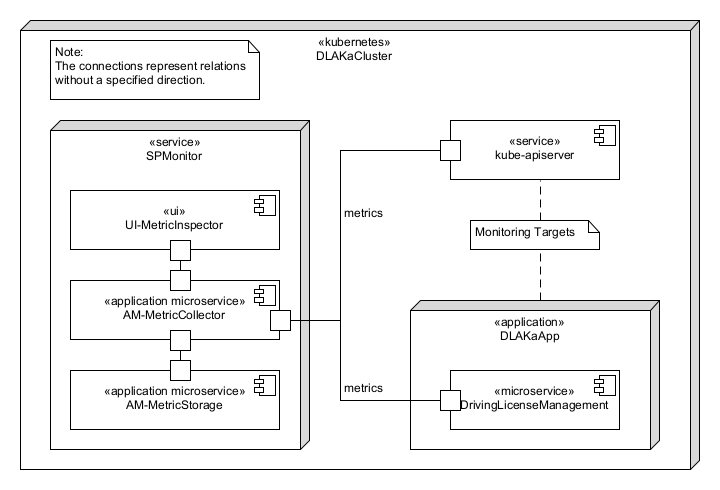
\includegraphics[width=\textwidth]{figures/6.2_abstract_sps_spmonitor.png}
  \caption{Abstract SystemPlusSoftware Architecture for SPMonitor}
  \label{fig:abstract_sps_spmonitor}
\end{figure}

Based on the analysis above, an abstract SPS (SystemPlusSoftware) architecture
was created for SPMonitor. The architecture can be seen in Figure
\ref{fig:abstract_sps_spmonitor}. In this architecture, no concrete tools are
considered. Instead, only abstract components and their interactions are
visualized. 
Every monitoring system, such as SPMonitor, requires a component to visualize data,
a data source, and a data sink. The visualization component will be
implemented by the user interface UI-MetricInspector. AM-MetricCollector is the
data source of SPMonitor and AM-MetricStorage is the data sink.
UI-MetricInspector provides the functionality of displaying the collected
metrics in dashboards and graphs. The microservice AM-MetricCollector is
responsible for collecting the metrics from DLAKaApp. It also provides an
interface for the user interface to access the stored values of the metrics.
The microservice AM-MetricStorage handles the storage of the metric values and
provides an interface to AM-MetricCollector for storing and accessing collected
metric values. The metric numDDL will be collected from the DLAKaApp's
AM-DrivingLicenseManagement and the metric MemUse will be collected
from the DLAKaCluster which is a Kubernetes cluster that provides the runtime
of the DLAKaApp. For the collection of the metrics, both the DLAKaApp and the
DLAKaCluster need to provide an interface through which AM-MetricCollector can
collect their respective metrics.

\subsection{Extension of the API Specification of AM-DrivingLicenseManagement}

The abstract SPS architecture defined in Figure
\ref{fig:abstract_sps_spmonitor} requires the DLAKaApp to provide two
interfaces that can be used by SPMonitor to collect metrics. The DLAKaCluster
running in Kubernetes already provides the required interface through an HTTP
endpoint at clusterURL/metrics. AM-DrivingLicenseManagement will have to be adapted with a similar endpoint. It
will also be hosted on the path /metrics and export metrics in the same format
as Kubernetes does. The actual format of the exported metrics might have to be
changed later if the data source that will be used requires a different format.
But the endpoint will conceptually still be the same. The format used by
Kubernetes is the Prometheus Metrics Format. In this format, each metric is
expressed as three lines of text. The first line provides information about the
meaning of the metric. The second line declares the type of metric. In the case
of numDDL, this is a counter which is a positive integer that can never
decrease. The last line contains the name of the metric and its value.
Optionally, the last line can also contain a set of labels with assigned
values. Labels are not used for the numDDL metric. 

The API specification of the metrics endpoint for AM-DrivingLicenseManagement can be seen in Listing
\ref{lis:api_spec_drivinglicensemanagement} which is written using the OpenAPI
standard. Line 3 defines the name of the API specification and line 4 the version of the API specification.
Under the paths attribute in line 5 the different API routes are defined.
Starting at line 6 the metrics endpoint for AM-DrivingLicenseManagement is defined.
This endpoint should only respond to requests that use the HTTP method GET as stated in line 7.
The endpoint has only one valid response whose description starts at line 9.
The only valid response from the metrics endpoint is sending a response with the HTTP status 200 (OK) as seen in line 9.
This response returns plain text that contains the metric data as described in lines 11 to 14.
lines 15 to 27 of the API specification provide two examples of valid response bodies of the metrics endpoint.
The first example of a response that contains metric data starts at line 16. The response body of this example
is described in lines 19 to 21. The second example is a response with no metric data which starts at line 22.
The response body of this example is described in lines 25 to 27.

\begin{lstlisting}[caption = {Partial API Specification of Application Microservice DrivingLicenseManagement}, label = {lis:api_spec_drivinglicensemanagement}, style = kit-cm, language=yaml]
openapi: 3.0.0
info:
  title: Partial API of Application Microservice DrivingLicenseManagement
  version: 1.0.0
paths:
  /metrics:
    get:
      responses:
        200:
          description: Success
          content:
            text/plain:
              schema:
                type: string
              examples:
                has_value: 
                  summary: The metric has a value
                  value: |
                    # HELP num_ddl Number of issued digital driving licenses
                    # TYPE num_ddl counter
                    num_ddl 42
                no_value: 
                  summary: The metric has no value
                  value: |
                    # HELP num_ddl Number of issued digital driving licenses
                    # TYPE num_ddl counter
                    num_ddl 0
\end{lstlisting}

The API diagram of AM-DrivingLicenseManagement also
needs to be adapted to provide the functionality of exporting metrics on an
HTTP endpoint. The API diagram represents the logical connection between
different endpoints in the style of Domain-Driven Design.

The changes to the API diagram consist of the integration of the SPMonitor
Library which will be developed to provide monitoring capabilities to
microservices implemented in Golang. The SPMonitor Library consists of three
entities and an interface. The entity MetricHandler exposes the method for
accessing the microservice's metrics through the method metrics. The
MetricHandler holds a reference to the entity MetricRegistry which stores a
list of all metrics that are being collected in the microservice. Each metric
implements the interface Metric that provides the basic properties needed by
all metrics which are a name and a help description. The only type of metric
needed by AM-DrivingLicenseManagement is a counter metric for the numDDL metric.
This is implemented as the entity CounterMetric that implements the Metric
interface. A counter metric holds an integer value that can only ever increase.
The entity IssuanceCollection holds a reference to a CounterMetric called
numDDL which will represent the numDDL metric. The adapted API diagram can be
seen in Figure \ref{fig:api_diagram_drivinglicensemanagement}. The
implementation of the SPMonitor Library and its integration into
AM-DrivingLicenseManagement was made by a student as part of his WASA2 practical
course thesis \cite{Am23}.

\begin{figure}[tb]
  \centering
  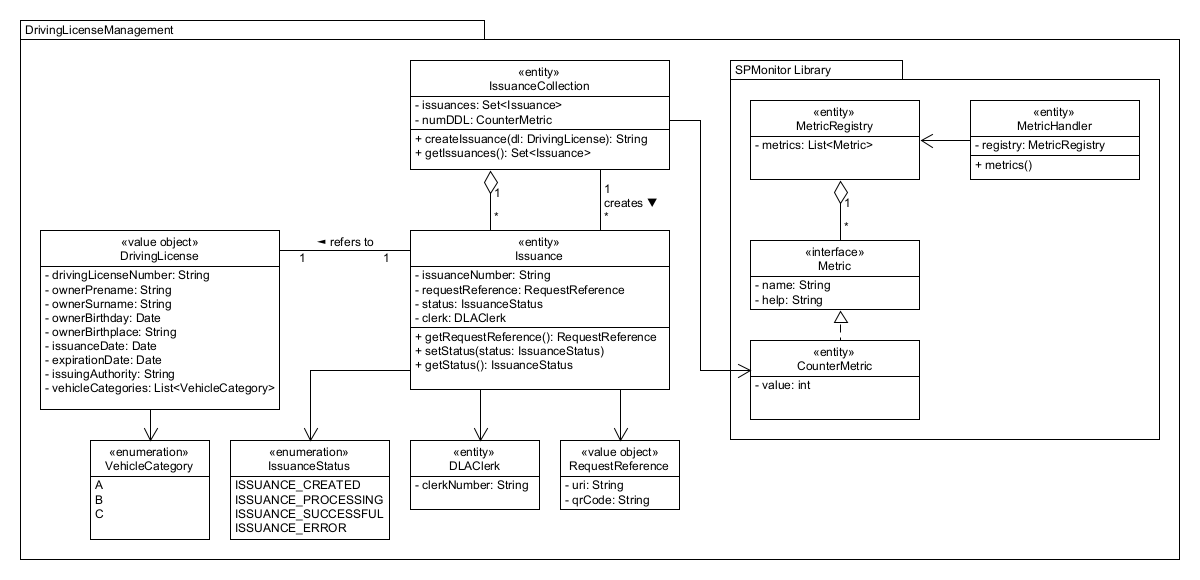
\includegraphics[width=\textwidth]{figures/6.3_api_diagram_drivinglicensemanagement.png}
  \caption{API Diagram Application Microservice DrivingLicenseManagement}
  \label{fig:api_diagram_drivinglicensemanagement}
\end{figure}

\subsection{Tool Selection Based on Capabilities and Requirements}

As explained in Chapter \ref{cha:technical_foundation}, a monitoring system
consists of three parts: The Data Source, Data Sink and a tool for
visualization. The data source is the core of a monitoring system. It is
responsible for collecting the monitoring data and dictates the needs for the
data sink as well as the possibilities for the visualization. Because of its
central role, the data source will be the first component of the monitoring
system that will be chosen and the rest of the monitoring system will be chosen
to best fit with and support the data source. The data source that will be
chosen must fulfill the requirements R3, R4, and R5 for SPMonitor that were
previously analyzed in Table \ref{tab:spmonitor_requirements}. The requirement
R3 is that the data source supports both the collection of metrics from
Kubernetes as well as from Golang microservices. R4 is that the data source
must support Kubernetes as a runtime and R5 is that the data source must have a
permissive license.

The data sources that will be compared according to the requirements in Table
\ref{tab:spmonitor_requirements} stem from the paper \enquote{A Survey on Observability of Distributed Edge {\&} Container-Based Microservices} by Usman
et al. \cite{UF+22}. Any entries that do not support metrics or are purely
research projects were eliminated. Lastly, the entry for Kibana was changed to
ELK for the ELK (ElasticSearch, LogStash, Kibana) stack. The complete overview
of all analyzed tools can be seen in Table \ref{tab:data_source_comparison}.

\begin{table}[]
  \centering
  \begin{tabular}{l|c|c|c|c}
    Name              & Purpose              & R3     & R4 & R5        \\
    \hline
    Apache SkyWalking & Performance          & \cmark & \cmark  & Free      \\
    Cilium            & Networking           & \cmark & \cmark  & Free      \\
    Datadog           & SaaS                 & \cmark & \cmark  & Paid      \\
    Dynatrace         & PaaS                 & \cmark & \cmark  & Paid      \\
    ELK               & Searching            & \cmark & \cmark  & Paid      \\
    Honeycomb         & Debugging            & \cmark & \cmark  & Paid      \\
    Instana           & Incidence Management & \cmark & \cmark  & Paid      \\
    \rowcolor{lightgray}
    Monasca           & MaaS                 & \cmark & \cmark  & Free      \\
    New Relic         & PaaS                 & \cmark & \cmark  & Paid      \\
    \rowcolor{lightgray}
    OpenTelemetry     & Monitoring           & \cmark & \cmark  & Free      \\
    \rowcolor{lightgray}
    Prometheus        & Monitoring           & \cmark & \cmark  & Free/Paid \\
    Scalyr            & PaaS                 & \cmark & \cmark  & Paid      \\
    SolarWinds        & PaaS                 & \cmark & \cmark  & Paid      \\
    Splunk            & Resilience           & \cmark & \cmark  & Paid      \\
    Sumo Logic        & Analytics            & \cmark & \cmark  & Paid      \\
  \end{tabular}
  \caption{Comparison of Data Sources}
  \label{tab:data_source_comparison}
\end{table}

The three final candidates for use in SPMonitor can be seen highlighted in Table \ref{tab:data_source_comparison}.
They are OpenTelemetry, Prometheus, and Monasca.
OpenTelemetry is a standalone solution for the collection of metrics. 
It provides many client libraries to instrument service for business metrics and can integrate
with most data sinks and visualization tools.
Prometheus is commonly used in combination with the LGTM (Loki Grafana Tempo Mimir) stack.
Loki is a service for handling logs, Tempo is responsible for handling traces, Grafana is used for visualization and Mimir provides
long-term storage for Prometheus. Prometheus itself is responsible for the collection of metrics.
As this work only considers metrics, the full setup would use Grafana for visualization, Prometheus as the data source, and Mimir
as the data sink. As Mimir only provides Prometheus with an interface to a storage system and is itself not one, it can be paired with MinIO
a free-to-use object storage system.
Monasca is a monitoring-as-a-service platform that collects metrics via the Monasca API.
Metrics can be collected by Monasca through the Monasca Kubernetes Agent as well as through
the Monasca clients. Monasca does not offer a user interface or metric storage
and also needs a messaging queue like RabbitMQ or Kafka.

From these three options, Prometheus together with Grafana, Mimir, and MinIO was chosen for SPMonitor.
Unlike OpenTelemetry, Prometheus provides easy integration with its data sink and visualization tool as
they were built to work together. OpenTelemetry on the other hand is a standalone solution meant to enhance
other tools that do not collect metrics themselves.
Monasca was ruled out because it would need to be paired with additional tools like Grafana,
which would also be used by Prometheus, as well as a messaging queue like RabbitMQ or Kafka and
a storage system. This would be more overhead compared to Prometheus.

\subsection{SPS Architecture of SPMonitor}

Based on the technology stack for SPMonitor consisting of Grafana, Prometheus, Mimir, and MinIO,
the abstract SPS architecture can be finalized into a concrete SPS architecture that is shown in
Figure \ref{fig:sps_spmonitor}. Grafana is used as the tool for the UI-MetricInspector
service from the abstract SPS architecture. Prometheus represents the microservice AM-MetricCollector
and the combination of Mimir and MinIO represents the microservice AM-MetricStorage.

\begin{figure}[tb]
  \centering
  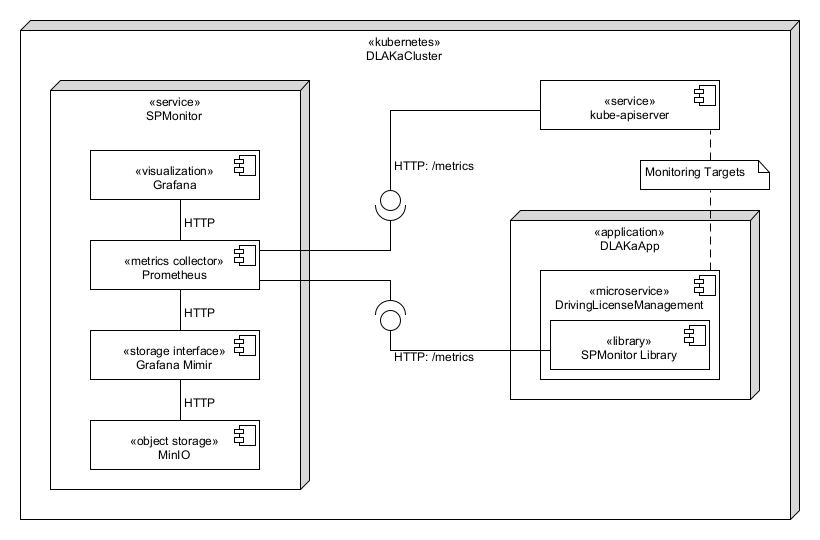
\includegraphics[width=\textwidth]{figures/6.4_sps_spmonitor.png}
  \caption{SystemPlusSoftware for SPMonitor}
  \label{fig:sps_spmonitor}
\end{figure}

\section{Implementation and Deployment}
\label{sec:impl_and_deployment}

With the design of SPMonitor finished it can be implemented and deployed.
SPMonitor will be implemented to be run as an Umbrella Helm Chart.
An Umbrella Helm Chart combines multiple Helm Charts into a single Helm Chart with one configuration file
for all Helm Charts.
The first step to achieving this was to create separate Helm Charts for the individual services
which would later be combined into an Umbrella Helm Chart.
Because most of the tools that are used by SPMonitor already provide suitable Helm Charts,
there was no implementation necessary, only the configuration of the Helm Charts. Mimir is the only tool
that required a new Helm Chart to be developed.
As stated earlier in the design, the SPMonitor Library has already been implemented and integrated into AM-DrivingLicenseManagement.

\subsection*{Prometheus Helm Chart}

\begin{figure}[tb]
\begin{lstlisting}[caption = {Prometheus Helm Chart Configuration}, label = {lis:prometheus_config}, style = kit-cm, language=yaml]
serverFiles:
  prometheus.yml:
    remote_write:
    - url: http://spmonitor-mimir-svc.default.svc.cluster.local:9009/api/v1/push
    scrape_configs:
      - job_name: kubernetes-nodes-cadvisor
        kubernetes_sd_configs:
          - role: node
            namespaces:
              names:
              - default
              - cm
      - job_name: spmonitor-scrape
        kubernetes_sd_configs:
        - role: endpoints
          namespaces:
            names:
            - default
            - cm
\end{lstlisting}
\end{figure}

The Helm Chart for Prometheus \cite{PRO-HELM} was configured first as it is the central service
of SPMonitor. The configuration of Prometheus focused on three things: the automatic discovery of services
that should be monitored, the connection to Mimir for persistency via the remote\_write URL, and the setup of a ServiceAccount
with permissions that allow Prometheus to access resources in the cluster that are needed for monitoring.
The configuration of Prometheus for the service discovery and remote\_write URL can
be seen in Listing \ref{lis:prometheus_config}.
The remote\_write URL is a single property in the configuration of the Prometheus
Helm Chart. The URL shown in Listing \ref{lis:prometheus_config} in line 4 points to the Mimir service
and is built up of three parts. The first part, spmonitor-mimir-svc, is the name
of the service resource for Mimir. The second part, default, is the namespace in which
the service lives. The third part, svc.cluster.local, is the default address
for services in the same cluster. Mimir receives metrics from Prometheus on port 9009
on the path /api/v1/push.
The service discovery is configured under the key scrape\_configs starting at line 5.
Prometheus works by regularly polling URL endpoints that have been configured
for metric collection, this is known as scraping, instead of having the services
push their metrics to Prometheus directly. The first scrape configuration with the name
kubernetes-node-cadvisor at line 6 scrapes pod metrics from the cluster via Kubernetes' cAdvisor service.
cAdvisor monitors the resource usage of containers in Kubernetes. The scraping is configured
via the role attribute which is set to node in line 8. This means that Prometheus will scrape the cAdvisor
endpoints on all pods in the namespaces that are given as a list via the namespaces attribute in line 9.
In the case of SPMonitor, the namespaces to be scraped are the default namespace and the namespace cm
which houses deployments made by the C\&M research group.

\begin{figure}[tb]
\begin{lstlisting}[caption = {Scrapable Endpoint Configuration for Prometheus}, label = {lis:scrape_endpoint_configuration}, style = kit-cm, language=yaml]
metadata:
  annotations:
    prometheus/path: /metrics
    prometheus/port: '8082'
    prometheus/scheme: http
    prometheus/scrape: 'true'
\end{lstlisting}
\end{figure}

The second scrape configuration, called spmonitor-scrape, starting at line 13 is configured to scrape URL
endpoints in the cluster that advertise themselves as scrapable. Prometheus looks for these
endpoints in the default and cm namespaces. Endpoints on services in Kubernetes can advertise themselves
as scrapable by setting the attributes seen in Listing \ref{lis:scrape_endpoint_configuration}.
The configuration shown in Listing \ref{lis:scrape_endpoint_configuration} is from
the metrics service of AM-DrivingLicenseManagement. This service exposes
metrics on the path /metrics on port 8082 via HTTP and signals Prometheus that it can
be scraped with the attribute prometheus/scrape being set to true.
The scrape configuration spmonitor-scrape is used to discover instances of AM-DrivingLicenseManagement
microservice that should be scraped for metrics.

\begin{figure}[tb]
\begin{lstlisting}[caption = {Prometheus ServiceAccount Configuration}, label = {lis:prometheus_rbac_config}, style = kit-cm, language=yaml]
kind: ClusterRole
metadata:
  name: prometheus-scrape
rules:
- resources:
    - nodes
    - nodes/metrics
    - endpoints
    - pods
  verbs:
    - get
    - list
    - watch
---
kind: ServiceAccount
metadata:
  name: prometheus-rbac
---
kind: Secret
metadata:
  name: prometheus-rbac-token
\end{lstlisting}
\end{figure}

Listing \ref{lis:prometheus_rbac_config} shows an excerpt of the configuration of the service account
required by Prometheus. The service account for Prometheus is called prometheus-rbac
and requires a ClusteRole, ClusterRoleBinding, and a Secret as additional Kubernetes resources.
A ClusterRole for Prometheus is set up starting at line 1
which bundles permissions into a named role which in this case is called prometheus-scrape.
This role permits the actions get, list, and watch defined under the attribute verbs at line 10
for the resources nodes, nodes/metrics, endpoints, and pods as defined under the attribute resources in line 5.
This allows Prometheus to execute the scrape configurations that were explained above.
This ClusterRole is bound to the ServiceAccount via a ClusterRoleBinding which is not shown.
Additionally, the service account also requires a service account access token to authenticate
with the Kubernetes API. This access token is stored in the Secret prometheus-rbac-token whose configuration starts at line 19.
The value for the access token is automatically set by Kubernetes when the resources
are installed into the cluster. To properly function, Prometheus requires two
CRDs (Custom Resource Definitions) to be installed in the cluster
that define custom Kubernetes resources. These two CRDs are called prometheus-probe
and prometheus-servicemonitor. They can be seen in the overview of the deployment resources
required by SPMonitor in Figure \ref{fig:spmonitor_resources}.

\subsection*{Grafana Helm Chart}

\begin{figure}[tb]
\begin{lstlisting}[caption = {Grafana Helm Chart Configuration}, label = {lis:grafana_config}, style = kit-cm, language=yaml]
datasources:
  datasources.yaml:
    datasources:
    - name: Prometheus
      type: prometheus
      url: http://spmonitor-prometheus-server.default.svc.cluster.local
      isDefault: true
dashboardsConfigMaps:
  default: "grafana-dashboards"
dashboardProviders:
  dashboardproviders.yaml:
    apiVersion: 1
    providers:
    - name: 'dlaka-dashboard-provider'
    - name: 'sp-dashboard-provider'
\end{lstlisting}
\end{figure}

The configuration of the Grafana Helm Chart \cite{GRA-HELM} focused on two things:
The connection to Prometheus as a default data source and the loading of pre-configured
dashboards at startup. An excerpt of the configuration of the Grafana Helm Chart
can be seen in Listing \ref{lis:grafana_config}.
Prometheus is configured as a default data source for Grafana by adding it to the list
of data sources in the Charts configuration under the attribute datasources at line 1.
This requires a name by which the data source can be identified by Grafana.
That name is set to Prometheus in line 4.
The type of data source that is being configured is also set to Prometheus at line 5.
The URL by which the data source can be reached is configured in line 6.
Whether or not it should be the default data source for Grafana is set to the value true in line 7.
The URL by which Grafana can reach Prometheus is configured similarly to the remote\_write
URL in the Prometheus configuration. The first part of the URL gives the name of the Kubernetes
service which in this case is the spmonitor-prometheus-server. The second part gives
the namespace of the service which is the namespace default and the third part, svc.cluster.local,
indicates that this is the URL of a service within the cluster.

\begin{figure}[tb]
\begin{lstlisting}[caption = {Grafana Dashboards ConfigMap}, label = {lis:grafana_dashboards_configmap}, style = kit-cm, language=yaml]
kind: ConfigMap
metadata:
  name: grafana-dashboards
data:
{{- range $path, $_ := .Files.Glob "resources/grafana/*.json" -}}
{{- $dashboardName := regexReplaceAll "(^.*/)(.*)\\.json$" $path "${2}" }}
  {{ $dashboardName }}.json: |
    {{ $.Files.Get $path | nindent 4 }}
{{- end -}}
\end{lstlisting}
\end{figure}

Grafana can export and import dashboards as JSON files. After SPMonitor was running
for the first time, the dashboards for DLAKa and SP were created and exported as JSON files.
The dashboards were created according to the metric definitions in Listings \ref{lis:metric_definition_memUse}
and \ref{lis:metric_definition_numDDL}.
To load the pre-configured dashboards into Grafana a ConfigMap called grafana-dashboards was used.
The ConfigMap was referenced in the Grafana configuration under the attribute dashboardConfigMaps.default at lines 8 and 9.
The configuration of the grafana-dashboards ConfigMap can be seen in Listing \ref{lis:grafana_dashboards_configmap}.
The ConfigMap uses Helm templating to load the contents of all JSON files in the directory
resources/grafana into properties of the ConfigMap where the name of the properties is taken
from the dashboard's filename without the .json extension.
This happens in lines 5 to 9.
To use the dashboards from the ConfigMap they are registered in the configuration file dashboardproviders.yaml
of Grafana in line 11. For each dashboard, an entry under the attribute providers in line 13 was made.
Each entry contains a name that Grafana will use to load the dashboard from the ConfigMap
where the dashboard is located as a property with the same name.
The pre-configured dashboard for DLAKa can be seen in Figure \ref{fig:spmonitor_dlaka_dashboard}
and the dashboard for SP in Figure \ref{fig:spmonitor_sp_dashboard}.

\begin{figure}[tb]
  \centering
  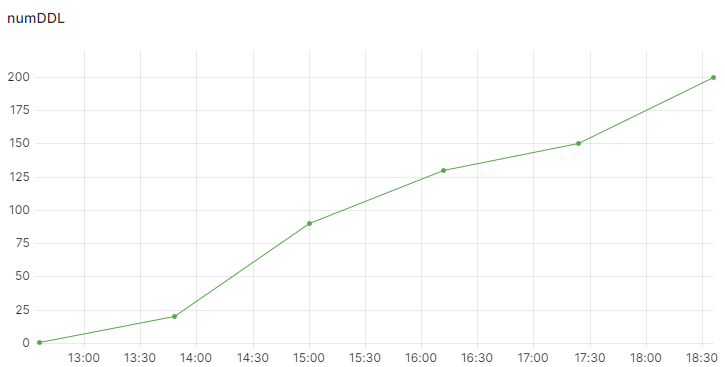
\includegraphics[width=0.6\textwidth]{figures/6.5_spmonitor_dlaka_dashboard.png}
  \caption{SPMonitor Dashboard for DLAKa}
  \label{fig:spmonitor_dlaka_dashboard}
\end{figure}

\begin{figure}[tb]
  \centering
  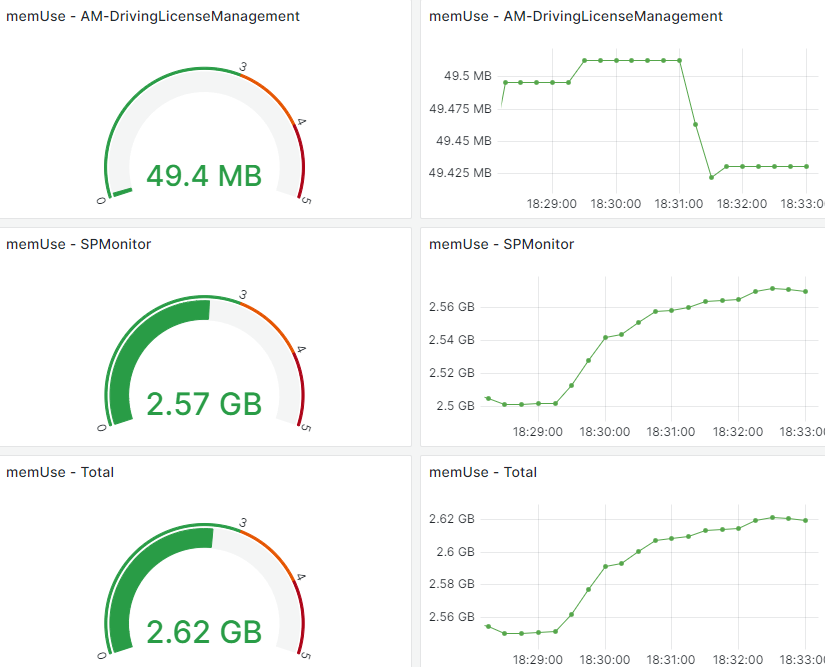
\includegraphics[width=0.7\textwidth]{figures/6.6_spmonitor_sp_dashboard.png}
  \caption{SPMonitor Dashboard for SP}
  \label{fig:spmonitor_sp_dashboard}
\end{figure}

\subsection*{Mimir Helm Chart}

Mimir can run in one of two deployment modes monolithic or microservice mode.
In the monolithic mode, Mimir runs as a single application that combines all the required functionality.
In the microservice mode, Mimir is split into multiple microservices that can be individually
scaled depending on demand. Because SPMonitor can only be deployed with constrained resources it was determined
that the microservice mode, which comes with a lot of overhead, was too resource expensive to use.
This meant that the monolithic mode would be used. While there is a Helm Chart available for Mimir
in microservice mode, there is only a Docker image \cite{MIM-IMG} available for Mimir in monolithic mode.
Therefore, the first task to running Mimir as a Helm Chart in monolithic mode was to use
the Docker image of Mimir and build a Helm Chart from it. This Chart is called spmonitor-mimir \cite{CM-G-SPM}.
The Chart consists of a Kubernetes Deployment and Service and requires a PVC
to be present that can be used by spmonitor-mimir to temporarily store data before forwarding it
to MinIO.

\begin{figure}[tb]
\begin{lstlisting}[caption = {SPMonitor's Mimir Deployment}, label = {lis:spmonitor_mimir_deployment}, style = kit-cm, language=yaml]
kind: Deployment
metadata:
  name: spmonitor-mimir
spec:
  replicas: 1
  template:
    spec:
      containers:
      - name: mimir
        image: grafana/mimir:latest
        ports:
          - containerPort: 8080
        envFrom:
        - secretRef:
            name: {{ .Values.s3.existingSecret }}
        args:
        - {{ printf "-common.storage.s3.endpoint=%s" .Values.s3.endpoint }}
        - {{ printf "-common.storage.s3.bucket-name=%s" .Values.s3.bucket_name }}
        - "-common.storage.backend=s3"
        - "-common.storage.s3.access-key-id=$(rootUser)"
        - "-common.storage.s3.secret-access-key=$(rootPassword)"
---
apiVersion: v1
kind: Service
metadata:
  name: spmonitor-mimir-svc
spec:
  ports:
  - port: 9009
    targetPort: 8080
\end{lstlisting}
\end{figure}

An excerpt of the Deployment can be seen in Listing \ref{lis:spmonitor_mimir_deployment}.
The Deployment takes the Docker image to run a single container from it which is configured in line 10.
The container is then configured to expose its port 8080 in line 12, use a PVC (PersistentVolumeClaim),
and is pre-configured with the bucket location used for storage in MinIO in lines 16 to 21.
The bucket location is pre-configured via runtime arguments to the executable of Mimir inside
of the container. The values needed for this are the endpoint and name of the bucket as well as
credentials for MinIO. For the credentials, the MinIO root access secret was used in lines 13 to 15.
Although this would not be secure in a production environment, it suffices for this research project.
The Service that was created simply maps the container's port 8080 to port 9009 on the Service
spmonitor-mimir-svc this is shown in lines 23 to 30.

\begin{figure}[tb]
\begin{lstlisting}[caption = {SPMonitor's Mimir Helm Chart Configuration}, label = {lis:mimir_config}, style = kit-cm, language=yaml]
pvcName: mimir-pvc
s3:
  endpoint: spmonitor-minio.default.svc.cluster.local:9000
  bucket_name: prometheus
  existingSecret: "minio-root-access"
\end{lstlisting}
\end{figure}

The Helm Chart for SPMonitor's Mimir requires a PVC (PersistentVolumeClaim) and an S3-like bucket to be configured.
The configuration of Mimir can be seen in Listing \ref{lis:mimir_config}.
Firstly, Mimir needs the name of the PVC that it can use for temporarily storing data which is configured in line 1.
Secondly, Mimir requires the configuration of the MinIO bucket location that consists
of the endpoint URL of the bucket in line 3, the bucket's name in line 4, and the name of a Secret that contains
the credentials to access MinIO in line 5.
Similar to other internally used URLs, the URL for the bucket endpoint consists of multiple parts.
The first part is the name of MinIO's service spmonitor-minio. The second part is the namespace
which is default. The third part, svc.cluster.local, indicates that this is a cluster internal URL
and finally, the endpoint is configured to send requests to MinIO on port 9000.

\subsection*{MinIO Helm Chart}

\begin{figure}[tb]
\begin{lstlisting}[caption = {MinIO Helm Chart Configuration}, label = {lis:minio_config}, style = kit-cm, language=yaml]
mode: standalone
existingSecret: "minio-root-access"
buckets:
  - name: prometheus
serviceAccount:
  name: "minio-sa"
persistence:
  existingClaim: "minio-pvc"
\end{lstlisting}
\end{figure}

The configuration of the MinIO Helm Chart \cite{MIN-HELM} focused on setting up
the storage needed for Prometheus and providing a pre-configured bucket into which Prometheus
can store its data via Mimir. An excerpt of MinIO's configuration can be seen in Listing \ref{lis:minio_config}.
MinIO has three different deployment modes Single-Node Single-Drive (standalone),
Single-Node Multi-Drive, and Multi-Node Multi-Drive. As the names suggest,
the Single-Node Single-Drive mode, also called standalone mode, runs MinIO on a single Kubernetes node with only one physical
drive while Single-Node Multi-Drive runs on one node with multiple physical drives and
Multi-Node Multi-Drive runs across multiple Kubernetes nodes with multiple drives.
For SPMonitor the standalone mode was chosen as only one drive is required for Prometheus
and advanced use cases for multiple drives or nodes like failover and replication were out of scope
for this thesis. Because of this MinIO was configured in standalone mode in line 1.
MinIO also requires a root access account with a username and password that is provided via a Secret called
minio-root-access in line 2. Next, the bucket for Prometheus is configured. Because of the scope of this thesis,
a simple bucket with the name prometheus and without any advanced configuration options was configured in lines 3 and 4.
Additionally, MinIO is configured to create its own ServiceAccount with the name minio-sa in lines 5 and 6 which is used
by MinIO to access PersistentVolumes (PV) and their associated PersistentVolumeClaims (PVC).
Lastly, MinIO is assigned a PVC which it can use to map its physical drives into. The PVC being used
was called minio-pvc and is configured in line 8.

\subsection*{SPMonitor Helm Chart}

\begin{figure}[tb]
\begin{lstlisting}[caption = {SPMonitor Umbrella Helm Chart}, label = {lis:spmonitor_helmchart}, style = kit-cm, language=yaml]
name: spmonitor
dependencies:
  - name: grafana
  - name: prometheus
  - name: spmonitor-mimir
    condition: persistency.enabled
  - name: minio
    condition: persistency.enabled
\end{lstlisting}
\end{figure}

With the individual Helm Charts configured, the Umbrella Helm Chart for SPMonitor
could be created. The Umbrella Helm Chart for SPMonitor can be seen in Listing \ref{lis:spmonitor_helmchart}.
The Charts for Grafana, Prometheus, spmonitor-mimir, and MinIO are listed as dependencies
in the Umbrella Helm Chart in lines 3 to 8. This allows all Charts to be configured from a single values.yaml file.
The dependencies spmonitor-mimir and minio are only include when a condition is met. This can be seen in lines 6 and 8.
The condition is that the flag persistency.enabled is set to true.
In the single configuration file for SPMonitor, the dependent Charts can be configured
by adding their configurations under a key with the same name as the name of the Chart listed in Listing \ref{lis:spmonitor_helmchart}.
The Chart for SPMonitor also has some additional configuration options.
Firstly, under the resources attribute the PVs and their PVCs for Mimir and MinIO can be configured.
This starts at line 1. For each PV and its PVC, the storage capacity and its location in the Node's filesystem
is configured. Secondly, there is a flag called persistency in line 12 which can be enabled or disabled.
Disabling the persistency flag removes Mimir and MinIO from the deployment of SPMonitor.

\begin{figure}[tb]
\begin{lstlisting}[caption = {SPMonitor Umbrella Helm Chart Configuration}, label = {lis:spmonitor_config}, style = kit-cm, language=yaml]
resources:
  mimir:
    storage:
      capacity: 1Gi
      hostPath:
        path: /data/mimir-pv/
  minio:
    storage:
      capacity: 1Gi
      hostPath:
        path: /data/minio-pv/
persistency:
  enabled: true
\end{lstlisting}
\end{figure}

\subsection*{Deployment of SPMonitor}

SPMonitor was manually deployed via ArgoCD to the bwcloud Kubernetes cluster which is a part
of the bwHPC (Baden-Württemberg High-Performance Computing) infrastructure that provides high-performance computing resources to research
institutes in the state of Baden-Württemberg. This program is run by the state of Baden-Württemberg.
To install an application into a Kubernetes cluster via ArgoCD two main steps need to be taken.
The first step is setting up a connection from ArgoCD to the repository or registry that contains
the Helm Chart and other Kubernetes resources that should be installed.
The second step is creating an application. An application in ArgoCD refers to a single active deployment.
The application requires a name, a sync policy, a source repository, a location and revision within the source repository, and a cluster destination.
ArgoCD can automatically update deployments when changes are applied to the application's source repository.
This is referred to as syncing the application. Because SPMonitor was only deployed once,
the sync policy was set to manual as no syncs were required. This means that the application
can still be synced with the source repository but only when a user starts the sync via the ArgoCD UI.
The configuration for the source repository will be described with the different applications that were deployed.
The bwcloud cluster was already pre-configured in ArgoCD as a destination.
An overview of all of the resources that were deployed for SPMonitor can be seen in Figure \ref{fig:spmonitor_resources}.
In addition to the components described in the implementation section, the deployment of SPMonitor
also consists of some additional resources.
As described in the implementation of the Prometheus Helm Chart the two CRDs required
by Prometheus were installed. Because the CRDs need to be installed before Prometheus can be installed,
the CRDs were manually installed into the cluster via ArgoCD as a separate application called spmonitor-crds.
The source repository for the CRDs is the same as for SPMonitor \cite{CM-G-SP}. The CRDs
are located in the repository in the directory resources/crds. This was set in ArgoCD as the path
in the repository for the spmonitor-crds application.
Similarly, the secrets required by SPMonitor were installed as a separate application called spmonitor-secrets.
The secrets for SPMonitor were separated into a different repository called SPMonitor Secrets \cite{CM-G-SPS}
that was used as the application's source repository.
With the CRDs and secrets set up, SPMonitor was installed into the cluster via ArgoCD.
The source repository for SPMonitor is the repository SPMonitor \cite{CM-G-SP}.
This repository also contains the Kubernetes resources for the additional resources required by SPMonitor
like the ServiceAccount with ClusterRole for Prometheus or the different PVs and PVCs.
Additionally, this repository also contains the configuration for a Kubernetes Ingress
and a Secret called ingress-secret.
The Ingress routes requests that reach the cluster to the different services of SPMonitor.

\begin{figure}[tb]
  \centering
  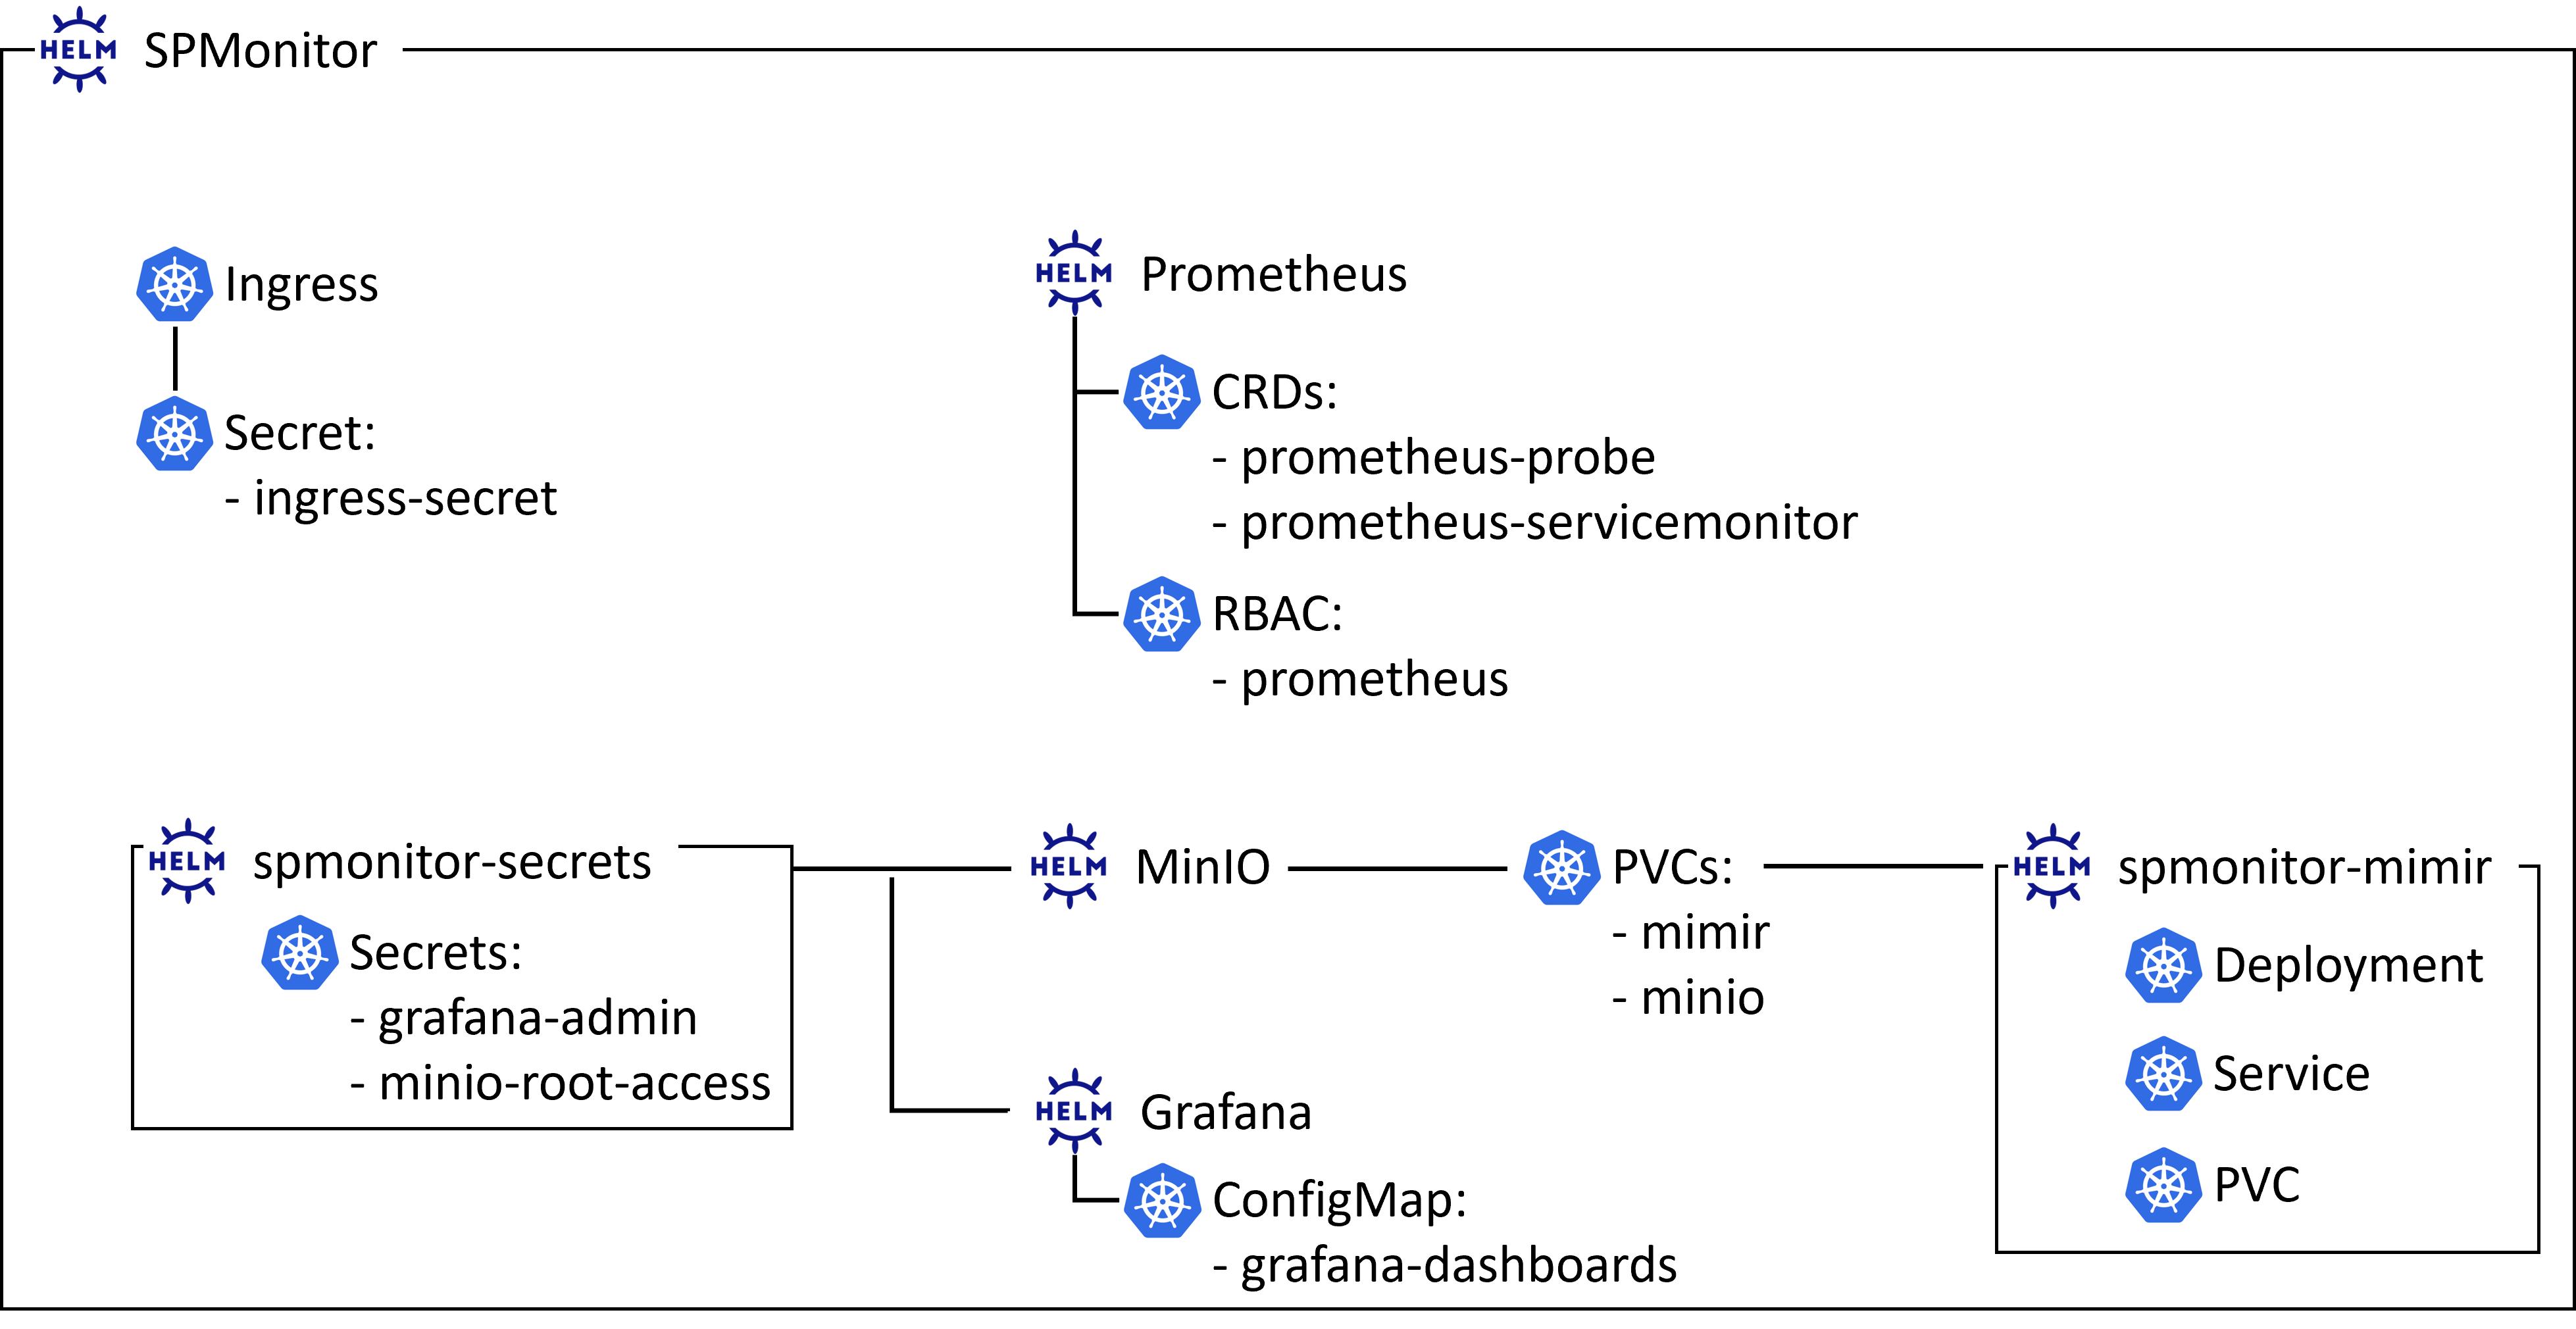
\includegraphics[width=0.7\textwidth]{figures/6.7_spmonitor_resources.png}
  \caption{SPMonitor Deployment Resources}
  \label{fig:spmonitor_resources}
\end{figure}
